%%%%%%%%%%%%%%%%%%%%%%%%%%%%%%%%%%%%%%%%%
% Programming/Coding Assignment
% LaTeX Template
%
% This template has been downloaded from:
% http://www.latextemplates.com
%
% Original author:
% Ted Pavlic (http://www.tedpavlic.com)
%
% Note:
% The \lipsum[#] commands throughout this template generate dummy text
% to fill the template out. These commands should all be removed when 
% writing assignment content.
%
% This template uses a Perl script as an example snippet of code, most other
% languages are also usable. Configure them in the "CODE INCLUSION 
% CONFIGURATION" section.
%
%%%%%%%%%%%%%%%%%%%%%%%%%%%%%%%%%%%%%%%%%

%----------------------------------------------------------------------------------------
%	PACKAGES AND OTHER DOCUMENT CONFIGURATIONS
%----------------------------------------------------------------------------------------

\documentclass{article}

\usepackage{fancyhdr} % Required for custom headers
\usepackage{lastpage} % Required to determine the last page for the footer
\usepackage{extramarks} % Required for headers and footers
\usepackage[usenames,dvipsnames]{color} % Required for custom colors
\usepackage{graphicx} % Required to insert images
\usepackage{subcaption}
\usepackage{listings} % Required for insertion of code
\usepackage{courier} % Required for the courier font
\usepackage{lipsum} % Used for inserting dummy 'Lorem ipsum' text into the template
\usepackage{amsmath}
\usepackage{bm}
\usepackage{array}
\usepackage{caption}

% Margins
\topmargin=-0.45in
\evensidemargin=0in
\oddsidemargin=0in
\textwidth=6.5in
\textheight=9.0in
\headsep=0.25in

\linespread{1.1} % Line spacing

% Set up the header and footer
\pagestyle{fancy}
\lhead{\hmwkAuthorName} % Top left header
\chead{\hmwkClass\ (\hmwkClassTime): \hmwkTitle} % Top center head
%\rhead{\firstxmark} % Top right header
\lfoot{\lastxmark} % Bottom left footer
\cfoot{} % Bottom center footer
\rfoot{Page\ \thepage\ of\ \protect\pageref{LastPage}} % Bottom right footer
\renewcommand\headrulewidth{0.4pt} % Size of the header rule
\renewcommand\footrulewidth{0.4pt} % Size of the footer rule

\setlength\parindent{0pt} % Removes all indentation from paragraphs

%----------------------------------------------------------------------------------------
%	CODE INCLUSION CONFIGURATION
%----------------------------------------------------------------------------------------

\definecolor{MyDarkGreen}{rgb}{0.0,0.4,0.0} % This is the color used for comments
\lstloadlanguages{Python} % Load Perl syntax for listings, for a list of other languages supported see: ftp://ftp.tex.ac.uk/tex-archive/macros/latex/contrib/listings/listings.pdf
\lstset{language=Python, % Use Perl in this example
        frame=single, % Single frame around code
        basicstyle=\small\ttfamily, % Use small true type font
        keywordstyle=[1]\color{Blue}\bf, % Perl functions bold and blue
        keywordstyle=[2]\color{Purple}, % Perl function arguments purple
        keywordstyle=[3]\color{Blue}\underbar, % Custom functions underlined and blue
        identifierstyle=, % Nothing special about identifiers                                         
        commentstyle=\usefont{T1}{pcr}{m}{sl}\color{MyDarkGreen}\small, % Comments small dark green courier font
        stringstyle=\color{Purple}, % Strings are purple
        showstringspaces=false, % Don't put marks in string spaces
        tabsize=5, % 5 spaces per tab
        %
        % Put standard Perl functions not included in the default language here
        morekeywords={rand},
        %
        % Put Perl function parameters here
        morekeywords=[2]{on, off, interp},
        %
        % Put user defined functions here
        morekeywords=[3]{test},
       	%
        morecomment=[l][\color{Blue}]{...}, % Line continuation (...) like blue comment
        numbers=left, % Line numbers on left
        firstnumber=1, % Line numbers start with line 1
        numberstyle=\tiny\color{Blue}, % Line numbers are blue and small
        stepnumber=5 % Line numbers go in steps of 5
}

% Creates a new command to include a perl script, the first parameter is the filename of the script (without .pl), the second parameter is the caption
\newcommand{\pythonscript}[2]{
\begin{itemize}
\item[]\lstinputlisting[caption=#2,label=#1]{#1.py}
\end{itemize}
}

%----------------------------------------------------------------------------------------
%	DOCUMENT STRUCTURE COMMANDS
%	Skip this unless you know what you're doing
%----------------------------------------------------------------------------------------

% Header and footer for when a page split occurs within a problem environment
\newcommand{\enterProblemHeader}[1]{
%\nobreak\extramarks{#1}{#1 continued on next page\ldots}\nobreak
%\nobreak\extramarks{#1 (continued)}{#1 continued on next page\ldots}\nobreak
}

% Header and footer for when a page split occurs between problem environments
\newcommand{\exitProblemHeader}[1]{
%\nobreak\extramarks{#1 (continued)}{#1 continued on next page\ldots}\nobreak
%\nobreak\extramarks{#1}{}\nobreak
}

\setcounter{secnumdepth}{0} % Removes default section numbers
\newcounter{homeworkProblemCounter} % Creates a counter to keep track of the number of problems
\setcounter{homeworkProblemCounter}{-1}

\newcommand{\homeworkProblemName}{}
\newenvironment{homeworkProblem}[1][Part \arabic{homeworkProblemCounter}]{ % Makes a new environment called homeworkProblem which takes 1 argument (custom name) but the default is "Problem #"
\stepcounter{homeworkProblemCounter} % Increase counter for number of problems
\renewcommand{\homeworkProblemName}{#1} % Assign \homeworkProblemName the name of the problem
\section{\homeworkProblemName} % Make a section in the document with the custom problem count
\enterProblemHeader{\homeworkProblemName} % Header and footer within the environment
}{
\exitProblemHeader{\homeworkProblemName} % Header and footer after the environment
}

\newcommand{\problemAnswer}[1]{ % Defines the problem answer command with the content as the only argument
\noindent\framebox[\columnwidth][c]{\begin{minipage}{0.98\columnwidth}#1\end{minipage}} % Makes the box around the problem answer and puts the content inside
}

\newcommand{\homeworkSectionName}{}
\newenvironment{homeworkSection}[1]{ % New environment for sections within homework problems, takes 1 argument - the name of the section
\renewcommand{\homeworkSectionName}{#1} % Assign \homeworkSectionName to the name of the section from the environment argument
\subsection{\homeworkSectionName} % Make a subsection with the custom name of the subsection
\enterProblemHeader{\homeworkProblemName\ [\homeworkSectionName]} % Header and footer within the environment
}{
\enterProblemHeader{\homeworkProblemName} % Header and footer after the environment
}

%----------------------------------------------------------------------------------------
%	NAME AND CLASS SECTION
%----------------------------------------------------------------------------------------

\newcommand{\hmwkTitle}{Project\ \#$1$} % Assignment title
\newcommand{\hmwkDueDate}{Monday,\ January\ 29,\ 2018} % Due date
\newcommand{\hmwkClass}{CSC411} % Course/class
\newcommand{\hmwkClassTime}{L2001} % Class/lecture time
\newcommand{\hmwkAuthorName}{Yuchen Wu} % Your name

%----------------------------------------------------------------------------------------
%	TITLE PAGE
%----------------------------------------------------------------------------------------

\title{
\vspace{2in}
\textmd{\textbf{\hmwkClass:\ \hmwkTitle}}\\
\normalsize\vspace{0.1in}\small{Due\ on\ \hmwkDueDate}\\
\vspace{0.1in}
\vspace{3in}
}

\author{\textbf{\hmwkAuthorName}}
%\date{} % Insert date here if you want it to appear below your name

%----------------------------------------------------------------------------------------

\begin{document}

\maketitle
\clearpage
%----------------------------------------------------------------------------------------
%	PROBLEM 0
%----------------------------------------------------------------------------------------

\begin{homeworkProblem}

\noindent \textit{\textbf{Introduction to CSC411 Project 1 Report and Instructions for Reproducing the Results}}

The submitted files for this project include a zip file named \texttt{faces.zip}; a pdf document named \texttt{faces.pdf} (this report); a Python script named \texttt{faces.py}; and a Latex source file named \texttt{faces.tex}

The zip file contains all the cropped out images downloaded from the FaceScrub dataset and used for completing project 1. It also contains figures and images used in this report. Please put the \texttt{figures} folder under the same directory with \texttt{faces.tex} to regenerate this pdf report if needed.

For reproducing the results, please first extract the zip file and put the \texttt{cropped\_images} folder under the same directory with the Python script, \texttt{faces.py}. All Python functions mentioned in this report can be found in the Python script, \texttt{faces.py}. Inside the \texttt{if \_\_name\_\_ == "\_\_main\_\_"} block, there are 10 functions (\texttt{part\_1} to \texttt{part\_8} ). The returned values or output of each functions produces the result for the corresponding part of the project. Please feel free to comment or uncomment any function inside this block to reproduce the result of certain parts.

Note that function \texttt{part\_1} in \texttt{faces.py} is used for downloading images from FaceScrub dataset, cropping the images and resizing it to 32 by 32 pixels. To run this function, please put the two text documents named \texttt{facescrub\_actors.txt} and \texttt{facescrub\_actresses.txt} under the same directory with the Python script, \texttt{faces.py}.


\end{homeworkProblem}
\clearpage

%----------------------------------------------------------------------------------------
%	PROBLEM 1
%----------------------------------------------------------------------------------------

% To have just one problem per page, simply put a \clearpage after each problem

\begin{homeworkProblem}

\noindent \textbf{\textit{Dataset Description}}

Figure~\ref{fig:p11} to Figure~\ref{fig:p13} provides nine examples of the images in the dataset and the corresponding cropped out faces. \\
Generally speaking, the dataset has decent annotation quality. The bounding boxes for most images are accurate and the cropped out faces are aligned with each other  (such as for Baldwin \#1, \#2 and \#3, as shown below in figure~\ref{fig:p11}). However, for a few images, the bounding boxes seems to be too small or too large (such as cropped out faces shown in figure~\ref{fig:p13}). In addition, for images in which the actor or actress is not facing the camera, the cropped-out faces are also sometimes not completely aligned (such as Baldwin \#31 and \#44 shown in figure~\ref{fig:p12} ). There are also a small number of cropped images (around 1\% in the dataset) that do not show faces, which is either because the original image does not include any face (such as Carell \#39 and Chenoweth \#13) or the bounding box is incorrect (such as Bracco \#89), as shown in figure~\ref{fig:p14}.

\begin{figure*}[h]
\begin{subfigure}{.35\textwidth}
  \centering
  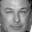
\includegraphics[width=.5\linewidth]{figures/cropped/baldwin1.jpg}
  \label{fig:c1}
\end{subfigure}%15
\begin{subfigure}{.35\textwidth}
  \centering
  
\includegraphics[width=.5\linewidth]{figures/cropped/baldwin2.jpg}
  \label{fig:c2}
\end{subfigure}%15
\begin{subfigure}{.35\textwidth}
  \centering
  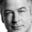
\includegraphics[width=.5\linewidth]{figures/cropped/baldwin3.jpg}
  \label{fig:c3}
\end{subfigure}%15

\begin{subfigure}{.35\textwidth}
  \centering
  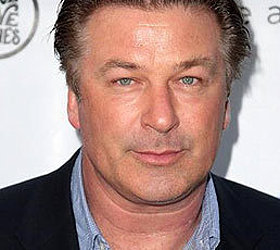
\includegraphics[width=.5\linewidth]{figures/uncropped/baldwin1.jpg}
  \caption{Baldwin \#1}
  \label{fig:c4}
\end{subfigure}%15
\begin{subfigure}{.35\textwidth}
  \centering
  
\includegraphics[width=.5\linewidth]{figures/uncropped/baldwin2.jpg}
  \caption{Baldwin \#2}
  \label{fig:c5}
\end{subfigure}%15
\begin{subfigure}{.35\textwidth}
  \centering
  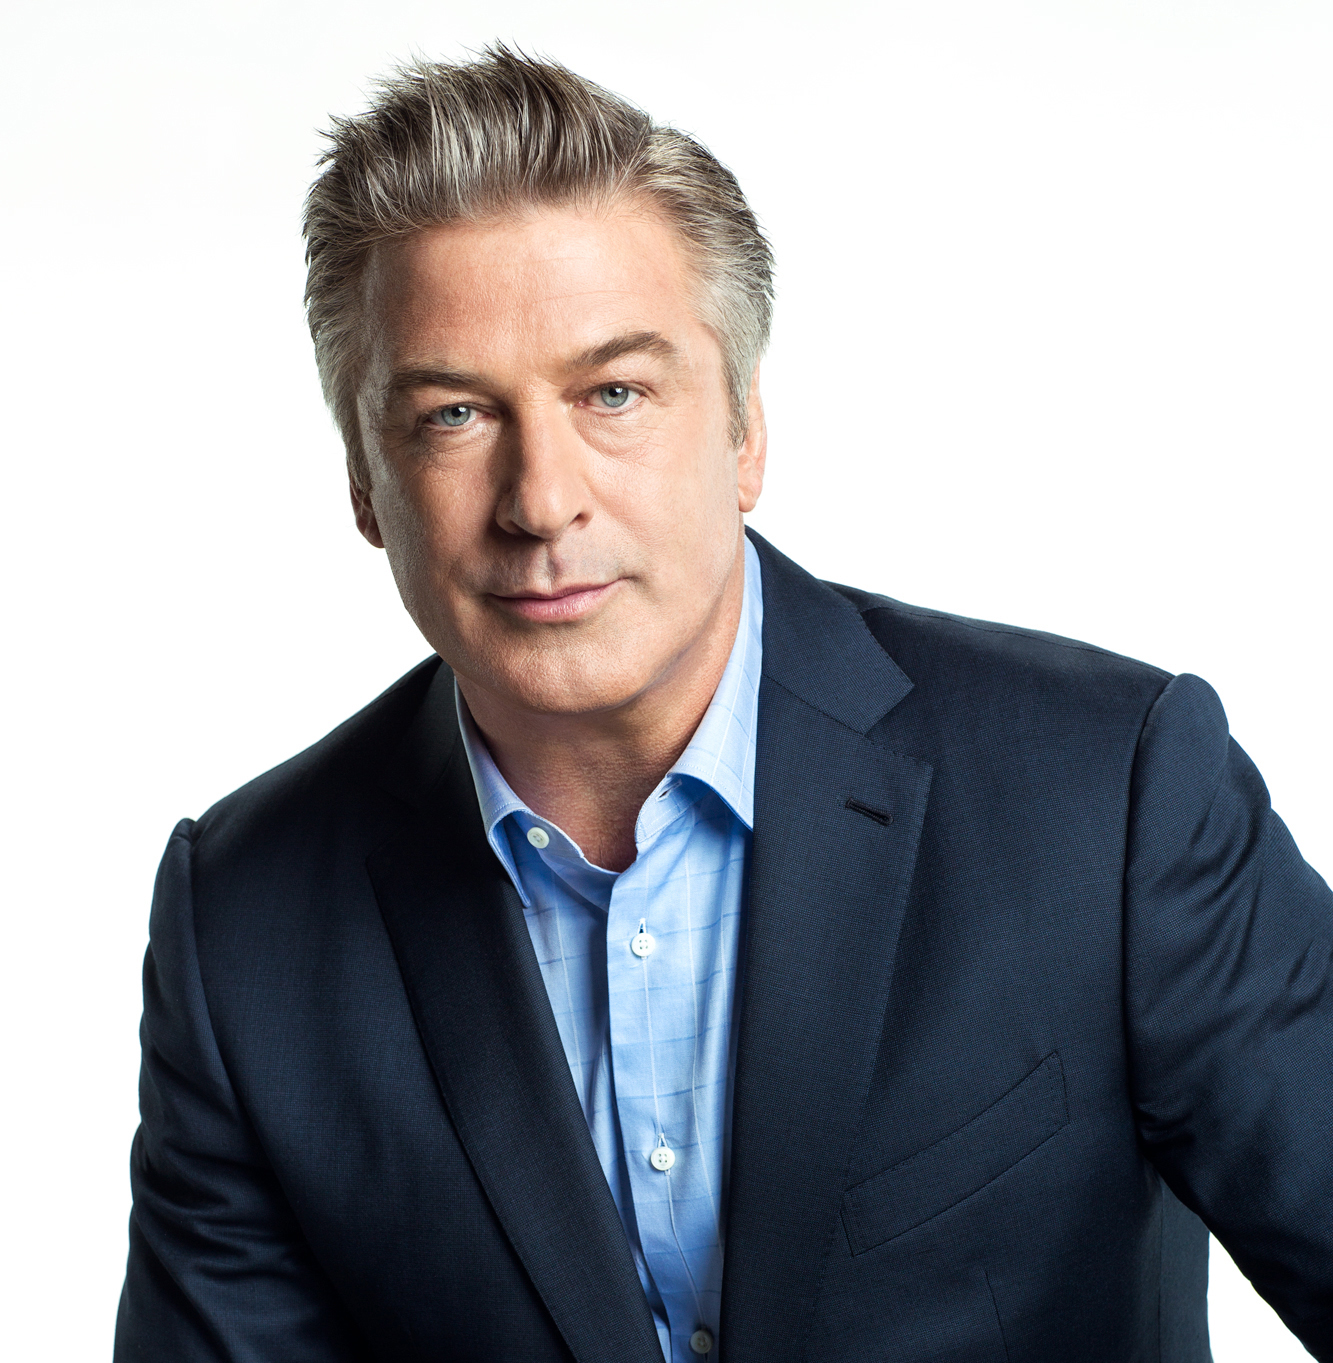
\includegraphics[width=.5\linewidth]{figures/uncropped/baldwin3.jpg}
  \caption{Baldwin \#3}
  \label{fig:c6}
\end{subfigure}%15
\caption{Examples of Correctly Cropped out Faces}
\label{fig:p11}
\end{figure*}


\begin{figure*}[h]
\begin{subfigure}{.35\textwidth}
  \centering
  
\includegraphics[width=.5\linewidth]{figures/cropped/baldwin31.jpg}
  \label{fig:c1}
\end{subfigure}%15
\begin{subfigure}{.35\textwidth}
  \centering
  
\includegraphics[width=.5\linewidth]{figures/cropped/baldwin44.jpg}
  \label{fig:c2}
\end{subfigure}%15

\begin{subfigure}{.35\textwidth}
  \centering
  
\includegraphics[width=.5\linewidth]{figures/uncropped/baldwin31.jpg}
  \caption{Baldwin \#31}
  \label{fig:c4}
\end{subfigure}%15
\begin{subfigure}{.35\textwidth}
  \centering
  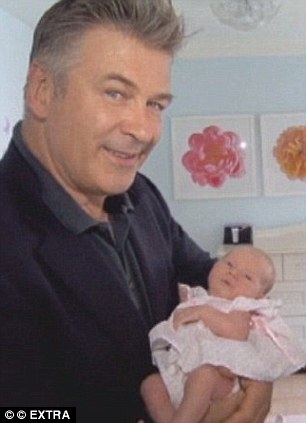
\includegraphics[width=.5\linewidth]{figures/uncropped/baldwin44.jpg}
  \caption{Baldwin \#44}
  \label{fig:c5}
\end{subfigure}%15
\caption{Examples of Cropped out Faces that are not Aligned with Most Faces}
\label{fig:p12}
\end{figure*}

\begin{figure*}[ht]
\begin{subfigure}{.35\textwidth}
  \centering
  
\includegraphics[width=.5\linewidth]{figures/cropped/baldwin34.jpg}
  \label{fig:c1}
\end{subfigure}%15
\begin{subfigure}{.35\textwidth}
  \centering
  
\includegraphics[width=.5\linewidth]{figures/cropped/drescher126.jpg}
  \label{fig:c2}
\end{subfigure}%15
\begin{subfigure}{.35\textwidth}
  \centering
  
\includegraphics[width=.5\linewidth]{figures/cropped/radcliffe129.jpg}
  \label{fig:c3}
\end{subfigure}%15

\begin{subfigure}{.35\textwidth}
  \centering
  
\includegraphics[width=.5\linewidth]{figures/uncropped/baldwin34.jpg}
  \caption{Baldwin \#34}
  \label{fig:c4}
\end{subfigure}%15
\begin{subfigure}{.35\textwidth}
  \centering
  
\includegraphics[width=.5\linewidth]{figures/uncropped/drescher126.jpg}
  \caption{Drescher \#126}
  \label{fig:c5}
\end{subfigure}%15
\begin{subfigure}{.35\textwidth}
  \centering
  
\includegraphics[width=.5\linewidth]{figures/uncropped/radcliffe129.jpg}
  \caption{Radcliffe \#129}
  \label{fig:c6}
\end{subfigure}%15
\caption{Examples of Cropped out Faces that are too Small or too Large}
\label{fig:p13}
\end{figure*}

\begin{figure*}[!ht]
\begin{subfigure}{.35\textwidth}
  \centering
  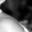
\includegraphics[width=.5\linewidth]{figures/cropped/bracco89.jpg}
  \label{fig:c1}
\end{subfigure}%15
\begin{subfigure}{.35\textwidth}
  \centering
  
\includegraphics[width=.5\linewidth]{figures/cropped/hader4.jpg}
  \label{fig:c2}
\end{subfigure}%15
\begin{subfigure}{.35\textwidth}
  \centering
  
\includegraphics[width=.5\linewidth]{figures/cropped/chenoweth13.jpg}
  \label{fig:c3}
\end{subfigure}%15

\begin{subfigure}{.35\textwidth}
  \centering
  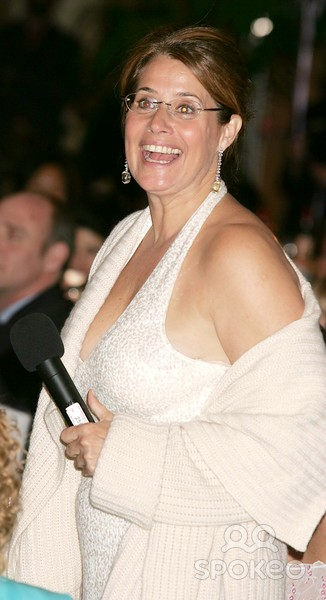
\includegraphics[width=.5\linewidth]{figures/uncropped/bracco89.jpg}
  \caption{Bracco \#89}
  \label{fig:c4}
\end{subfigure}%15
\begin{subfigure}{.35\textwidth}
  \centering
  
\includegraphics[width=.5\linewidth]{figures/uncropped/carell39.jpg}
  \caption{Carell \#39}
  \label{fig:c5}
\end{subfigure}%15
\begin{subfigure}{.35\textwidth}
  \centering
  
\includegraphics[width=.5\linewidth]{figures/uncropped/chenoweth13.jpg}
  \caption{Chenoweth \#13}
  \label{fig:c6}
\end{subfigure}%15
\caption{Examples of  Error Cropped out Faces}
\label{fig:p14}
\end{figure*}

\end{homeworkProblem}
\clearpage
%----------------------------------------------------------------------------------------

%	PROBLEM 2
%----------------------------------------------------------------------------------------

\begin{homeworkProblem}

\noindent \textbf{\textit{Dataset Separation Algorithm}}

According to the requirement, 90 images are needed in total for each actor (the training set requires 70 face images per actor/actress, the validation set requires 10 face images per actor/actress, and the test set requires 10 face images per actor/actress). Due to difference in total number of images for each actor/actress downloaded from the FaceScrub dataset, the algorithm first selects 90 images randomly among downloaded images of each actor/actress. Then, it randomly chooses 10 images and another 10 images from the 90 images of each actor and put them into the \textit{validation} set and the \textit{test} set, respectively. The rest of images are put into the \textit{training} set. Randomization is used in this algorithm to avoid potential bias. This algorithm was implemented in function \texttt{part\_2}. The function returns 3 dictionaries storing the separated training set, validation set and test set, respectively. (Please run function \texttt{part\_2} in \texttt{faces.py} to see its returning examples.) The values in each dictionary are the filenames of the selected pictures and the corresponding keys are labels (i.e. name of corresponding actors/actresses). 

The separated sets represented in dictionaries obtained from function \texttt{part\_2} can then be converted to corresponding feature matrices (\textbf{X}) and label matrices (\textbf{Y}) through helper function \texttt{create\_set} when needed. The function \texttt{create\_set} takes two input parameters. The first parameter is one of the sets (training, validation or test) returned from \texttt{part\_2} and the second parameter is another dictionary that stores the value of labels to be used (e.g. -1\&1 or 0\&1 for a binary classifier). The function \texttt{create\_set} is explicitly called in function \texttt{part\_3\_classifier} to get the feature matrices (\textbf{X}) and label matrices (\textbf{Y}) of training, validation and test set. Please run \texttt{part\_3\_classifier} and see what it returns if needed.

\end{homeworkProblem}
\clearpage
%----------------------------------------------------------------------------------------

%	PROBLEM 3
%----------------------------------------------------------------------------------------

\begin{homeworkProblem}

\noindent \textbf{\textit{Binary Classification Using Linear Regression: Distinguish Pictures of Alec Baldwin from Pictures of Steve Carell}}

\textit{The Cost function}\\
Linear regression is used, as required, to build the classifier. The hypothesis $h_{\theta}(x)$ is 
\begin{align*}
h_{\theta}(x) &= h_{\theta}(x_0,x_1,x_2,...,x_{1024})\\
&=x_0\theta_0+x_1\theta_1+x_2\theta_2+...x_{1024}\theta_{1024}\\
&=\bm{\theta^T}\textbf{x}
\end{align*}

where $x_0=1$ and $x_k$ is the $k^{th}$ pixel of the picture. Since each image after being cropped and resized is 32 by 32, so there are 1024 pixels in total for each image (i.e. $k = 1$ to $1024$). In addition, the input images are divided by 255.0 so that all inputs are in the 0 to 1 range.

The cost function chosen to minimize was the sum of squared differences between the expected outputs and the actual outputs,
\begin{align*}
J(\bm{\theta}) = \dfrac{1}{2m}\sum_{i=1}^{m}(h_{\theta}(x^{(i)})-y^{(i)})^2
\end{align*}
(Note: The expected output (label) for Alec Baldwin is -1 and 1 for Steve Carell. $m$ is the number of inputs.)\vspace*{0.5cm}

\textit{Performance of the classifier}\\
Value of cost function on the training set: $f(x)_{training\ set} = 0.000374 \pm 0.000044$\\
Value of cost function on the validation set: $f(x)_{validation\ set} = 0.207773 \pm 0.042181$\\
Performance of the classifier on the training set:  $100.0\% \pm 0.000000\%$\\
Performance of the classifier on the validation set:  $90.00\% \pm 5.477226\% $\\
(Note: this result was produced by function \texttt{part\_3} and was obtained from 5 trials with different training and validation sets in same size.)\vspace*{0.5cm}

\textit{Code of the function used for computing the output of the classifier}\\
The code of the function used to compute the output of the classifier is shown below (\texttt{faces.py} from line 204 to 211):
\begin{lstlisting}[language=python]
def output(x,theta,anti_classify_act):
"""
Compute the output of the Binary Classifier with a threshold of 0
Take:
    x: input
    theta: trained weights
    anti_classify_act: a dictionary that stores the correct label of each actor
        for this part: {-1 : 'Alec Baldwin', 1:'Steve Carell'}
Return:
    result: output of the classifier i.e. name of the corresponding actor
"""
    result = []
    for k in np.matmul(theta,x):
        if k > 0 : # if h(x)>0 then classify as 'Steve Carell' for this part
            result.append(anti_classify_act[1])
        else: # otherwise classify as 'Alec Baldwin' for this part
            result.append(anti_classify_act[-1])
    return result
\end{lstlisting}
To classify the faces, a threshold of 0 is used to differentiate the two classes.
\begin{align*}
  Output(x)=\begin{cases}
               -1, h_{\theta}(x)<0\\
               1, h_{\theta}(x)>0\\
            \end{cases}
\end{align*}
In this case, $-1$ corresponds to "Alec Baldwin" and $1$ corresponds to "Steve Carell".\vspace{0.5cm}

\textit{Parameter selections}\\
The initial value of $\theta$s, learning rate $\alpha$ and stopping condition $EPS$ for gradient descent were selected carefully in order for the system to work. Since in this part, the system is only expected to work and over-fitting issues are not yet considered, maximum number of iteration for gradient descent process was set to a large number (100000) to avoid early stopping.
\begin{itemize}
\item Select initial value of $\theta$s: \\
Since the cost function is convex. It is expected that initial value of $\theta$s are selected such that the initial value of the cost function is relatively small. In other words, it is expected that the initial value of $\theta$s are close to the desired value so that the cost function could converge to global minimum quickly during gradient descent process.\\
Table~\ref{tab:long} below shows the initial value of function with initial $\theta$s under normal distribution with different variance. The result was generated from function \texttt{part\_3}. Note: there were 5 trials for each initial distribution of $\theta$s.
\begin{center}
\captionof{table}{Initial Value of Cost Function under Different Initial Value of $\theta$s}
\label{tab:long}
\begin{tabular}{ || m {2cm} | m {6cm}||}
\hline
Initial $\theta$s
&Initial value of the cost function\\

\hline
$N(0,0.0)$
&$140.00 \pm 0.00$\\
\hline
$N(0,0.0001)$
&$139.98 \pm 0.02$\\
\hline
$N(0,0.001)$
&$139.95 \pm 0.32$\\
\hline
$N(0,0.01)$
&$142.38 \pm 4.35$\\
\hline
$N(0,0.1)$
&$464.42 \pm 273.86$\\

\hline\hline
\end{tabular}
\end{center}
Based on the result, all initial $\theta$s were selected to be zeros because it, in general, minimized the initial value of the cost function.

\item Select learning rate $\alpha$ for gradient descent:\\
\begin{figure*}[!ht]
\begin{subfigure}{.5\textwidth}
  \centering
  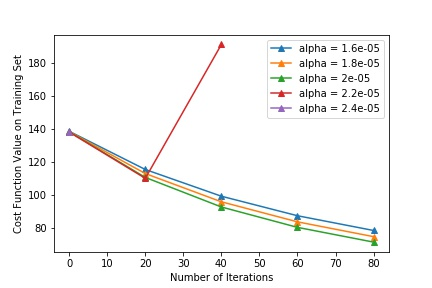
\includegraphics[width=.9\linewidth]{figures/part3f1.jpg}
  \label{fig:c1}
\end{subfigure}%15
\begin{subfigure}{.5\textwidth}
  \centering
  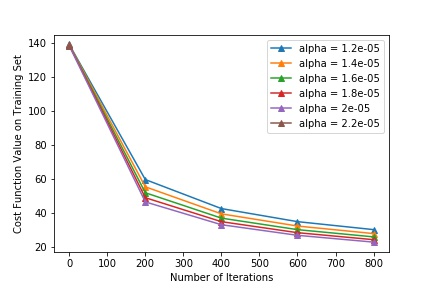
\includegraphics[width=.9\linewidth]{figures/part3f2.jpg}
  \label{fig:c2}
\end{subfigure}%15

\caption{Value of Cost Function vs. Number of Iterations}
\label{fig:p31}
\end{figure*}

The learning rate $\alpha$ is expected to be small enough such that the cost function could converge to its minimum after performing gradient descent. However, it also should not be too small because in that case it would lead to slow convergence. Figure~\ref{fig:p31} shows the change in value of the cost function during gradient descent with different learning rates. (Note: The initial $\theta$s were all set to be zero based on previous observations.)

The result shows that the system diverges when learning rate is greater than $2\times10^{-5}$. The rate of convergence does not vary a lot for the learning rate $\alpha$ ranging from $1.2\times10^{-5}$ to $2\times10^{-5}$. Therefore, the learning rate was eventually set to $1.5\times10^{-5}$ to ensure convergence and maximize rate of convergence to a certain extent.

\item Select stopping condition for gradient descent (EPS): \\
The stopping condition EPS was selected to be a fixed number, 1e-5, which was given in function \texttt{grad\_descent} provided in lecture.

\end{itemize}


\end{homeworkProblem}
\clearpage

%----------------------------------------------------------------------------------------
%	PROBLEM 4
%----------------------------------------------------------------------------------------

\begin{homeworkProblem}

\noindent \textbf{\textit{(a) View}} \textit{$(\bm{\theta}_1,...,\bm{\theta}_n)$} \textbf{\textit{as an Image}} 

$\theta$s (except $\theta_0$) were reshaped to (32,32) for visualization. Figure~\ref{fig:p41}  below shows the $\theta$s obtained by training using the full training dataset (70 images for each actor).
\begin{figure*}[!ht]
\centering
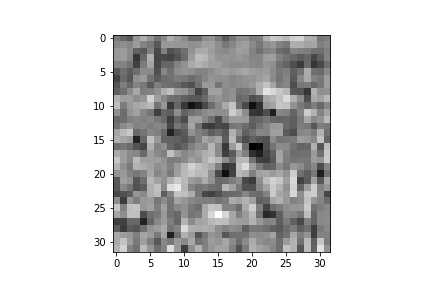
\includegraphics[scale=0.6]{figures/part4f1.jpg}
\caption{$\theta$s from Full Training Set}
\label{fig:p41}
\end{figure*}

Figure~\ref{fig:p42}  below shows the $\theta$s obtained by training using a training set that contains only two images of each actor.
\begin{figure*}[!ht]
\centering
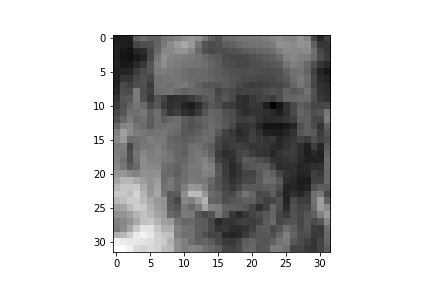
\includegraphics[scale=0.6]{figures/part4f2.jpg}
\caption{$\theta$s from Training Set Containing Two Images of each Actor}
\label{fig:p42}
\end{figure*}

Note: For this part, all parameters used are same as those in Part 3. The maximum iterations for gradient descent  were set to be 100000 (a fairly large number) to avoid early stopping.
\clearpage

\noindent \textbf{\textit{(b) Produce both kinds of Visualizations}}

Using the full training set with same setup (stopping condition EPS = 1e-5, learning rate $\alpha$=1.5e-5), the two kinds of visualizations can be produced by stopping the Gradient Descent process earlier and later in the process or initialing $\theta$s using different strategies. 
\begin{itemize}
\item Stopping the Gradient Descent process earlier and later in the process.\\
Figure~\ref{fig:p43} (left) shows the image of $\theta$s when the gradient descent process was stopped at $100^{th}$ iteration. Figure~\ref{fig:p43} (right) shows the image of $\theta$s when the gradient descent process was stopped at $10000^{th}$ iteration. All $\theta$s were initialized to be zero.
\begin{figure*}[!ht]
\begin{subfigure}{.5\textwidth}
  \centering
  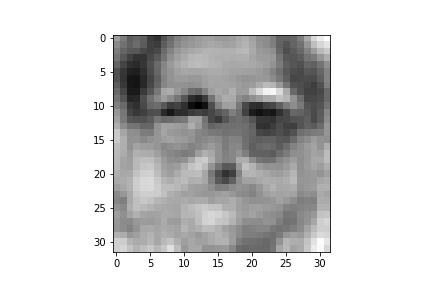
\includegraphics[width=.9\linewidth]{figures/part4f5.jpg}
  \label{fig:c1}
  \caption{Earlier (100th iteration)}
\end{subfigure}%15
\begin{subfigure}{.5\textwidth}
  \centering
  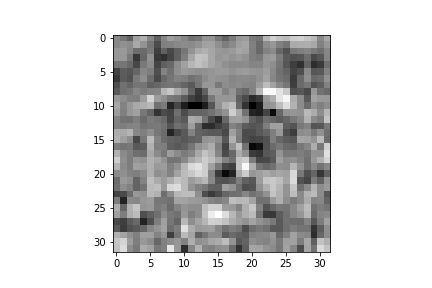
\includegraphics[width=.9\linewidth]{figures/part4f6.jpg}
  \label{fig:c2}
  \caption{Later (10000th iteration)}
\end{subfigure}%15

\caption{Stopping the Gradient Descent process earlier and later}
\label{fig:p43}
\end{figure*}

The result shows that, when all the $\theta$s are zero initially, the image of $\theta$s after being trained tends to look more like a face when the gradient descent process stops relatively earlier.

\item Initializing the $\theta$s under normal distribution with different standard deviation.

Figure~\ref{fig:p44} (left) shows the image of $\theta$s when the initial values of $\theta$s are under normal distribution with 0.0001 standard deviation and 0 mean; Figure~\ref{fig:p44} (right) shows the image of $\theta$s when the initial values of $\theta$s are under normal distribution with 0.1 standard deviation and 0 mean. The maximum number of iteration was fixed at 1000.
\begin{figure*}[!ht]
\begin{subfigure}{.5\textwidth}
  \centering
  
\includegraphics[width=.9\linewidth]{figures/part4f3.jpg}
  \label{fig:c1}
  \caption{$\mu=0$ $\sigma=0.0001$}
\end{subfigure}%15
\begin{subfigure}{.5\textwidth}
  \centering
  
\includegraphics[width=.9\linewidth]{figures/part4f4.jpg}
  \label{fig:c2}
   \caption{$\mu=0$ $\sigma=0.1$}
\end{subfigure}%15

\caption{ Initialize values of $\theta$s under normal distribution with different mean and variance}
\label{fig:p44}
\end{figure*}

It can be seen from the two images that, when the gradient descent stops early in the process (i.e. early stopping), the image tends to look like a face when the standard deviation of  initial $\theta$s are small, which means that $\theta$s are very close to a constant (zero in this case) initially.

\end{itemize}



\end{homeworkProblem}
\clearpage

%----------------------------------------------------------------------------------------

%	PROBLEM 5
%----------------------------------------------------------------------------------------

\begin{homeworkProblem}

\noindent \textbf{\textit{Binary Classification Using Linear Regression: Classify the Actors as Males or Females}}

For this part, the training set contains 70 images of each actor/actress and the validation set contains 10 images of each actor/actress listed below:
\begin{itemize}
\item Females: 'Lorraine Bracco', 'Peri Gilpin', 'Angie Harmon'
\item Males: 'Alec Baldwin', 'Bill Hader', 'Steve Carell'
\end{itemize}

The test set contains 10 images of each actor/actress listed below:
\begin{itemize}
\item Females: 'Kristin Chenoweth', 'Fran Dresher', 'America Ferrera'
\item Males: 'Gerard Butler', 'Daniel Radcliffe', 'Michael Vartan'
\end{itemize}

Females are labelled as $-1$ and males are labelled as $1$.\vspace{0.5cm}

\textit{Over-fitting Demonstration}\\
Figure~\ref{fig:p51} shows the performance of the classifiers on the training and validation sets as well as on the test set verses the size of the training set. (10 trials were run for each different training set size with different images in the training set.)

Note that for this part, the parameters (stopping condition $EPS$, learning rate $\alpha$ and initial values of $\theta$s) were selected in the same way as in Part 3. The maximum number of iteration was set to a fairly large number (10000) to avoid early stopping. It was also noticed that stopping earlier in the gradient descent could sometimes prevent the model from over-fitting to the training set. This observation is discussed in detail in Part 7.
\begin{figure*}[!ht]
\centering
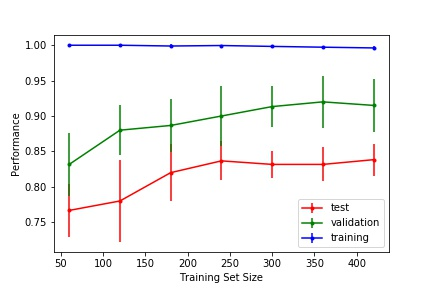
\includegraphics[scale=0.8]{figures/part5f1.jpg}
\caption{Performance of the classifiers on the training, validation and test set vs. different training set size\\($\alpha=0.000005$; $EPS = 1e^-5$; Initial $\theta=0s$; $Max\ Num.\ of\ Iteration = 10000$)}
\label{fig:p51}
\end{figure*}

The above result shows that the classifier always has highest accuracy on the training set (nearly  100\%), although the performance decreases slightly as the size of training set grows. Although performance of the classifier on the validation set is always higher than which on the test set, performance on both sets gets improved as the size of training set becomes larger. The result indicates that, when the training set is relatively small, the model tends to be over-fitting to the training set because its performance on the validation set (80\%-85\%) and test set (75\%-80\%) is much worse than on the training set. As the training set size becomes larger (about 70 images for each actor), performance on the validation set increases to around 90\%, which indicates that the model is less over-fitting to the images used in the training set. However, since the performance on the test set (i.e. another six actors) is much less than on the training set (80\%-85\%), the model is still over-fitting to the gender of the six actors/actresses used in the training set. \vspace{0.5cm}

\textit{Report the performance on the test set}\\
The performance of the classifier on the 6 actors who are not included in $act$ (i,e performance on the test set as shown above) is $83.8333\%\pm2.2423\%$ when using the full training set (70 images for each actor, 420 in total). The performance would decrease when using training set with smaller size.

\end{homeworkProblem}
\clearpage

%----------------------------------------------------------------------------------------
%	PROBLEM 6
%----------------------------------------------------------------------------------------

% To have just one problem per page, simply put a \clearpage after each problem

\begin{homeworkProblem}

\noindent \textbf{\textit{(a) Compute $\dfrac{\partial J}{\partial \theta_{pq}}$}}

As required, The cost function is still the sum of squared differences between the expected outputs and the actual outputs:
\begin{align*}
J(\bm{\theta}) = \sum_{i=1}^m(\sum_{j=1}^k(\theta^Tx^{(i)}-y^{(i)})_j^2)
\end{align*}
So, the partial differentiation with respect to $\theta_{pq}$ can be computed by chain rule,
\begin{align*}
\dfrac{\partial J}{\partial \theta_{pq}} &= \dfrac{\partial (\sum_{i=1}^m(\sum_{j=1}^k(\theta^Tx^{(i)}-y^{(i)})_j^2))}{\partial\theta_{pq} }\\
&=\sum_{i=1}^m\dfrac{\partial (\sum_{j=1}^k(\theta^Tx^{(i)}-y^{(i)})_j^2)}{\partial\theta_{pq} }\\
&=\sum_{i=1}^m2\cdot(\sum_{h=1}^n \theta^T_{qh} x_{h}^{(i)} - y_q^{(i)})\cdot \dfrac{\partial (\sum_{h=1}^n \theta^T_{qh} x_{h}^{(i)} - y_q^{(i)})}{\partial\theta_{pq} }\\
&=2\cdot\sum_{i=1}^m(\sum_{h=1}^n \theta^T_{qh} x_{h}^{(i)} - y_q^{(i)})\cdot x_p^{(i)}\\
&= 2\cdot \sum_{i=1}^m ( x_p^{(i)} \cdot (\sum_{h=1}^n \theta^T_{qh} x_{h}^{(i)} - y_q^{(i)}) )\\
\end{align*}

Note: the dimension of $\theta$, $x^{(i)}$ and $y^{(i)}$ were mentioned in the project instructions.

\clearpage
\noindent \textit{\textbf{(b) Derivative of J(}$\bm{\theta}$\textbf{) with respect to all the components of }$\bm{\theta}$}

Define $m$ as the number of training examples; $n=1025$ as the number of features (pixels) of each image with an additional "1"; $k$ as the number of possible output of the model. Then, $\bm{\theta}$ is a $n\times k$ matrix, $\textbf{X}$ is a $n\times m$ matrix and $\textbf{Y}$ is a $k\times m$ matrix.\\

\textit{Method 1}

It can be shown that
\begin{align*} 
(2X(\theta^TX-Y)^T)_{pq} &= 2\cdot \sum_{i=1}^m X_{pi}(\theta^TX-Y)^T_{iq}\\
&= 2\cdot \sum_{i=1}^m X_{pi}(\theta^TX-Y)_{qi}\\
&= 2\cdot \sum_{i=1}^m X_{pi}((\theta^TX)_{qi}-Y_{qi})\\
&= 2\cdot \sum_{i=1}^m X_{pi}(\sum_{h=1}^n \theta^T_{qh} X_{hi} - Y_{qi})\\
&= 2\cdot \sum_{i=1}^m ( x_p^{(i)} \cdot (\sum_{h=1}^n \theta^T_{qh} x_{h}^{(i)} - y_q^{(i)}) )\\
&= \dfrac{\partial J}{\partial \theta_{pq}} \text{ (Computed in Part 6 (a))}
\end{align*}

Therefore, the derivative of $J(\theta)$ with respect to all the components of $\theta$ can be written in matrix form as $2X(\theta^TX-Y)^T$.\\

\textit{Method 2}

The cost function $J(\bm{\theta}) = \sum_{i=1}^m(\sum_{j=1}^k(\theta^Tx^{(i)}-y^{(i)})_j^2)$  can be written in matrix form as 
\begin{align*}
tr((\theta^TX-Y)(\theta^TX-Y)^T) &= tr(\theta^TXX^T\theta - YX^T\theta - \theta^TXY^T+YY^T)
\end{align*}
According to general formula of matrix differentiation, the gradient of $J(\bm{\theta})$ with respect to $\bm{\theta}$ is: 
\begin{align*}
\nabla_{\bm{\theta}}J(\bm{\theta})&=2XX^T\theta-2XY^T=2X(X^T\theta-Y^T)=2X(\theta^TX-Y)^T
\end{align*}

\clearpage
\noindent \textit{\textbf{(c) Implement the cost function from Part 6(a) and its vectorized gradient function}}\\
The code below shows the implementation of the cost function from Part 6(a) and its vectorized gradient function in Python. (\texttt{faces.py} from line 645 to 651)
\begin{lstlisting}[language=python]
def part_6_f(x, y, theta):
	"""
	Quadratic loss function for part 6. 
	Take:
		x: the input data (images)
		y: the label of input data
		theta: the weight matrix
	Return:
		Quadratic loss function derived in (b) method 2
	"""
    cost = np.matmul(theta.transpose(),x)-y 
    #the cost function in matrix form as derived in (b) Method 2
    return np.trace(np.matmul(cost,cost.transpose())) 

def part_6_df(x, y, theta):
	"""
	Compute the gradient of the quadratic loss function for part 6 wrt thetas. 
	Take:
		x: the input data (images)
		y: the label of input data
		theta: the weight matrix
	Return:
		The gradient matrix of loss function wrt thetas derived in (b)
	"""
    cost = np.matmul(theta.transpose(),x)-y 
    return 2*np.matmul(x,cost.transpose())
\end{lstlisting}

\clearpage
\noindent \textit{\textbf{(d) Compute the gradient using finite-difference approximations}}\\
\textit{Code for computing the gradient components using finite differences}\\
Code shown below is used for computing the gradient components using finite differences and compare them to the gradient computed using function in Part 6(b) (\texttt{faces.py} from line 690 to 712). Relative error is used to compared the approximated values to the output of the gradient function. The formula for relative error is
\begin{center} $Err(Approx,Output)=|Approx-Output|/(|Approx|+|Output|)$. \end{center}
\begin{lstlisting}[language=python]
def part_6d_finite_diff_approx(f,x,y,theta,h,p,q):
	"""
	Compute the gradient component theta_pq
	Take:
   	 f: the cost function    x: input features    y: labels    theta: weights
	Return:
		the partial derivative computed using finite difference approximation 
			wrt theta_pq
	"""
    thetah = theta.copy()
    # increase theta_pq by h
    thetah[p][q] += h
    return (f(x, y, thetah)-f(x, y, theta))/h
def part_6_d_error(f,x,y,theta,h,p,q):
	"""
	Compare the error of the pq component of gradient wrt theta between the finite 
		difference approximation and value obtained from function in Part 6b
	Take:
   		f: the cost function    x: input features    y: labels
   		theta: weights    h: finite difference
   		p and q: coordinates
   	Return:
   		error: Relative error between approximation and the actual value
	"""
    approx = part_6d_finite_diff_approx(f, x, y, theta,h,p,q)
    actual = part_6_df(x, y, theta)[p][q]
    #Compute the relative error between approximation and the actual value
    #The formula for relative error is error(a,b)=|a-b|/(|a|+|b|)
    error = np.abs(approx-actual)/(np.abs(approx)+np.abs(actual))
    return error
\end{lstlisting}

When $h$ is set to $10^{-8}$, the mean relative error between the approximated gradient and the gradient obtained from formula in (b) is around $10^{-7}$, which indicates that the vectorized gradient function works. The reason for selecting $h$ to be $10^{-8}$ is discussed below.
\clearpage
\textit{Select the Value of $h$}
\begin{figure*}[!ht]
\centering
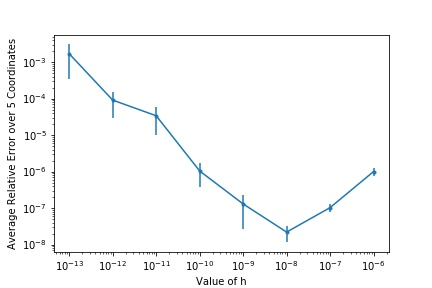
\includegraphics[scale=0.65]{figures/part6f1.jpg}
\caption{Relative Error between Finite Difference Approximation and True Gradient}
\label{fig:p61}
\end{figure*}

Figure~\ref{fig:p61} above shows the relative error, computed using function \texttt{part\_6\_d\_error} above, between the gradient computed using the function in Part 6(b) and the finite-difference approximations along 5 coordinates with different values of $h$. From the plot, the relative error between finite-difference approximation and the true gradient is minimized when $h$ is around  $10^{-8}$. Although based on definition, the error should converge to zero as $h$ goes to zero, it ,in fact, increases when $h$ becomes too small due to numerical issues (e.g. arithmetic underflow).

\end{homeworkProblem}
\clearpage
%----------------------------------------------------------------------------------------
%	PROBLEM 7
%----------------------------------------------------------------------------------------

\begin{homeworkProblem}

\noindent \textit{\textbf{Multi-class Classification Using Linear Regression: Run Gradient Descent on the Set of Six Actors/Actresses }}

\textit{Parameter Selections}\\
Similar to Part (3), the initial values of $\theta$s, learning rate $\alpha$ and stopping condition $EPS$ for gradient descent were first selected carefully in order for the system to work. For this part, the stopping condition $EPS$ was still chosen to be 1e-5, which was given in function $\texttt{Grad\_Descent}$ provided in lecture. Based on result in Part 3, the initial value of $\theta$s  were chosen to be zeros because that made the initial value of the cost function to be relatively small (i.e. close to the minimum). Also, for the learning rate, several values were tested and shows in figure~\ref{fig:p71} below. 
\begin{figure*}[!ht]
\begin{subfigure}{.5\textwidth}
  \centering
  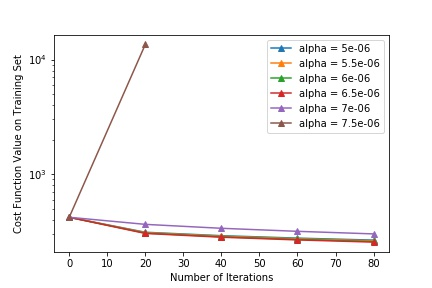
\includegraphics[width=.9\linewidth]{figures/part7f1.jpg}
  \label{fig:c1}
\end{subfigure}%15
\begin{subfigure}{.5\textwidth}
  \centering
  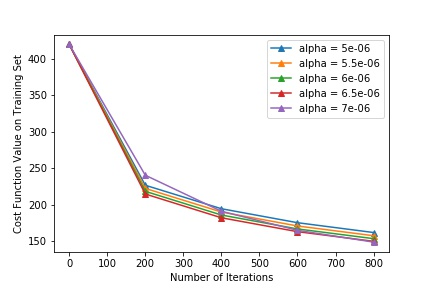
\includegraphics[width=.9\linewidth]{figures/part7f2.jpg}
  \label{fig:c2}
\end{subfigure}%15

\caption{Value of Cost Function vs. Number of Iterations}
\label{fig:p71}
\end{figure*}

The result shows that the system diverges when learning rate is greater than $7\times10^{-6}$. The rate of convergence does not vary a lot for the learning rate $\alpha$ ranging from $5\times10^{-6}$ to $6.5\times10^{-6}$. Therefore, the learning rate was eventually set to $6\times10^{-6}$ to ensure convergence and maximize rate of convergence to a certain extent.
\begin{figure*}[!ht]
\centering
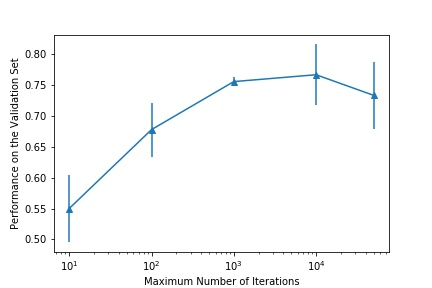
\includegraphics[scale=0.65]{figures/part7f3.jpg}
\caption{Performance of the classifiers on the validation set vs. number of iterations}
\label{fig:p73}
\end{figure*}
Another important parameter is the number of iterations. Consider that the model may be over-fitting to the training set, the Gradient Descent process is expected to stop when the classifier gets best performance on the validation set rather than when the cost function is minimized. Figure~\ref{fig:p73} shows the performance of the classifiers the validation set after different number of iterations. It shows that the performance of the classifiers on the validation set is optimized at around 10000 iterations.\vspace{0.5cm}

\textit{Performance of the classifier}\\
Performance of the classifier on the training set:  $98.8889\% \pm 0.2970\%$\\
Performance of the classifier on the validation set:  $76.6667\% \pm 4.9065\% $\\
Note: this result was produced from function \texttt{part\_7} and was got through 3 trials with different training set (size = 420) and validation set (size = 60).\vspace*{0.5cm}

\textit{Output of the Model}\\
To produce the output of the model, firstly, the maximum value among the output vector of the hypothesis function $h_{\theta}(x)$ is considered as 1, other values are considered as 0. Then, the vector containing only 1 and 0s is compared with the label of each actor and the actor with the same label vector is the output of the model. For example, assume that the output of the hypothesis function is [0.6,0.8,0.3,0.5,0.2,0.6]. The maximum value is 0.8 in this vector so that the output of the hypothesis function is considered as [0,1,0,0,0,0]. Then, the actor with label [0,1,0,0,0,0] is the output of the model.

\end{homeworkProblem}
\clearpage
%----------------------------------------------------------------------------------------
%	PROBLEM 8
%----------------------------------------------------------------------------------------

\begin{homeworkProblem}

\noindent \textit{\textbf{Visualization of }$\bm{\theta}$\textbf{s for Multi-class Classification}}

Figure~\ref{fig:p81}  shows the images of each row of $\theta$s and the corresponding actors/actresses.

\begin{figure*}[!ht]
\begin{subfigure}{.35\textwidth}
  \centering
  
\includegraphics[width=.5\linewidth]{figures/part8f1.jpg}
  \caption{Angie Harmon}
  \label{fig:c1}
\end{subfigure}%15
\begin{subfigure}{.35\textwidth}
  \centering
  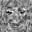
\includegraphics[width=.5\linewidth]{figures/part8f2.jpg}
  \caption{Lorraine Bracco}
  \label{fig:c2}
\end{subfigure}%15
\begin{subfigure}{.35\textwidth}
  \centering
  
\includegraphics[width=.5\linewidth]{figures/part8f3.jpg}
  \caption{Peri Gilpin}
  \label{fig:c3}
\end{subfigure}%15

\begin{subfigure}{.35\textwidth}
  \centering
  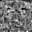
\includegraphics[width=.5\linewidth]{figures/part8f4.jpg}
  \caption{Alec Baldwin}
  \label{fig:c4}
\end{subfigure}%15
\begin{subfigure}{.35\textwidth}
  \centering
  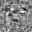
\includegraphics[width=.5\linewidth]{figures/part8f5.jpg}
  \caption{Bill Hader}
  \label{fig:c5}
\end{subfigure}%15
\begin{subfigure}{.35\textwidth}
  \centering
  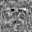
\includegraphics[width=.5\linewidth]{figures/part8f6.jpg}
  \caption{Steve Carell}
  \label{fig:c6}
\end{subfigure}%15

\caption{Parameter Visualization for each Actor/Actress}
\label{fig:p81}
\end{figure*}

\end{homeworkProblem}
\clearpage

%----------------------------------------------------------------------------------------

\end{document}